% -*- coding: utf-8 -*-


\documentclass{oblivoir}
\usepackage{kotex}
\usepackage{indentfirst}
\usepackage{graphicx}
\DeclareGraphicsExtensions{.pdf,.png,.jpg}

\title{Assignment 1.
	K-means Algorithm}
\author{정원철}
\begin{document}
\maketitle
\begin{center}
\begin{tabular}{l r}
	학 번 : & 20113560 \\
	학 년 : & 4학년 \\
	과 목 : & 휴먼인터페이스 영상 \\
	교 수 : & 홍병우 교수님 \\
	전 공 : & 컴퓨터공학과 \\
	대 학 : & 중앙대학교
\end{tabular}
\end{center}
\begin{flushright}
	\begin{center}
 Mathematical Foundations for Computer Vision and Machine Learning,\\
 Computer Science Department, Chung-Ang University,\\
 20113560, Won-Cheol Jeong,\\
 prof. Byung-Woo Hong
 	\end{center}
\end{flushright}

\tableofcontents
\newpage


\section{개요 \label{ss:add}}
K-mean은 알고리즘은 기준 값으로부터 인접한 주변 값들로 주어진 전체 데이터를 K개의 클러스터로 분류하는 알고리즘이다.\\

본 과제에서는 이미지 색을 데이터로 K-means를 적용, 분류하는 이미지 분할 프로그램을 구현한다. 목표는 이미지 내 대표적인 K개의 색으로 이미지 전체의 색을 대체함으로써 이미지를 분석하기 좋은 표현으로 바꾸며, 간단한 압축기술을 구현하는 것이다.

\section{알고리즘 기술 \label{ss:add}}
본 과제의 전체 프로그램 과정은 다음과 같다.
\begin{enumerate}
	\item 이미지를 불러들이고 각 픽셀을 RGB값으로 수치화한다. 이는 이미지 프로세싱을 위하여 수치화된 데이정를 필요로 하는데 이미지의 픽셀을 Red, Green, Blue의 가산으로 수치화 표현할 수 있기 때문이다.
	\item 픽셀 RGB값들로 K-means를 시행한다. K-means의 과정은 아래에서 확인한다.
	\item 결과값인 클러스터 그룹 내의 픽셀들을 대표값으로 색 통일한다.\\
\end{enumerate}


K-means 알고리즘의 스텝은 다음과 같다.
\begin{enumerate}
	\item 초기값을 설정한다. 본 과제에서는 초기화 알고리즘인 Fogy 알고리즘을 기본으로 초기값을 설정했다.
	\item[-] Fogy알고리즘은 데이터 전체에서 K개의 데이터를 무작위로 선택하고, 이 데이터들이 초기 클러스터의 중심값이 되도록 설정한다.
	\item 각 데이터에서 가장 가까운 클러스터 중심값을 찾는다. 이 클러스터에 데이터를 포함한다. 모든 픽셀에 대하여 반복한다.
	\item[-] 가장 가까운 관계(유사도)는 유클리드 기하학의 거리로 사용했다.
	\item 클러스트를 대표하는 중심값을 새로 계산한다.
	\item 기존 중심값과 새로운 중심값이 다르다면 변화가 있는 것이다. 변화한다면 1부터 과정을 반복한다. 변화하지 않는 것(수렴)이 종료조건이다.
\end{enumerate}



\section{구현기술 \label{ss:add}}
\begin{figure}
	\begin{center}
		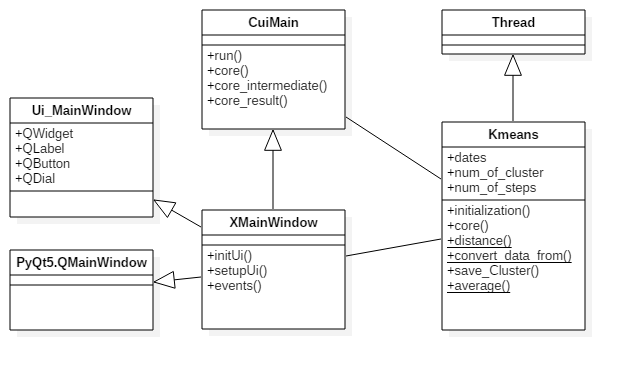
\includegraphics[scale=0.5]{uml.png}
	\end{center}
\end{figure}

본 파이썬 프로그램은 3개의 클래스로 구성되어져 있으며 로직은 2개로 흐른다. 우선 3개의 클래스는 CUI, GUI, Kmeans라는 이름을 가지고 있다. Kmeans클래스는 본 프로그램의 핵심 코어로 K-means 알고리즘으로 구현되있다. CUI클래스는 외부 이미지의 입력으로부터 K-means에 수치 데이터 입력까지의 로직, K-means의 출력으로부터 본 프로그램의 결과를 도출하는 과정으로 구현되었다. CUI클래스가 이 로직을 터미널 인터페이스상에서 한다면, GUI는 그래픽 인터페이스에서 이 로직을 실행한다. GUI는 CUI클래스의 데코레이트 패턴으로 구현되었으며 PyQt5를 상속받아 레이아웃과 이벤트를 구현했다.\\

본 프로그램은 인수의 수를 기준으로 CUI와 GUI를 구분한다. CUI로의 실행은 python run1.py \{이미지명.확장자\} \{클러스터 수(k)\} \{루프 제한 정도\}이다. GUI로의 실행은 python run1.py 로 인수 없음이 되겠으며, 직관적인 인터페이스로 구현되었다.\\
Kmeans 클래스와 인터페이스를 담당하는 클래스(CUI/GUI)는 별개의 스레드를 생성함으로 K-means 프로세싱 중에도 이벤트 처리들은 별도로 계속된다.




\section{단점 및 개선방안 \label{ss:add}}
K-means 알고리즘은 인접성으로 클러스터들을 분류한다. 그리고 이 인접성에 따라 각 클러스터의 사이로 경계선이 그어진다. K-means의 문제는 만약 초기 K개의 중심 값이 치우쳐져 있다면 전체의 범위보다 지역적 범위 내에서 경계선이 생성되는 과정이 반복되고, 그 과정에 종료조건이 발생한다는 것이다.
\newline


즉 K-means 알고리즘은 지역적수렴의 문제를 안고 있다. 이의 방법은 초기값의 선정이 지역적 수렴구에 들지 않도록 해야함을 말한다. 이를 개선하기 위한 방법으로 초기값이 지엽적이지 않게 흩뿌리는 초기값 설정 개선방안을 생각할 수 있다. 효과적인 알고리즘 중 하나로 K-means++가 있다. 이는 다음 추가구현에서 보인다. 
\newline

다음으로는 K-means의 프로세싱 과정 중 경계를 부드럽게 가져가는 것이다. 이 역시 지역수렴을 극복하는 방법 중 하나이다. 퍼지 C-means에 대해서 다음 추가구현에서 보인다.
\newline

또 다른 단점으로는 K-means의 구현 과정에 중심값과 다른 모든 값들 사이의 유사도를 계산한다는 것이다. 이는 이 알고리즘의 복잡도를 증가시키는 주된 원인이다. 이를 개선하는 방안으로 데이터들을 트리 구조로 정렬하여 비교횟수를 줄이는 방법을 생각할 수 있다. 또 기본 유사도를 측정하는 방법인 유클리드 거리 계산을 다른 방법으로 바꾸는 것을 생각할 수도 있다. 앞선 방법은 유사도 탐색 알고리즘인 M-tree, Kd-tree 구조나 MAM색인 등을 알아보게 되었지만 구현에는 미치지 못하였다.


\section{추가구현 \label{ss:add}}

\section{구현결과 성능측정 \label{ss:add}}

\section{개발환경 \label{ss:add}}
\begin{enumerate}
	\item[-] OS: Windows10 x64
	\item[-] PL: Python3.6 (및 3.5, 2.7에서 동작)
	\item[-] Library: PyQt5
	\item[-] Doc: LaTex, gnuplot, starUML
	\item[-] DVCS: git (https://github.com/NarciSource/Graphics.Project)
	\item[-] Tools: VisualStudio2017, TeXstudio, Qt Designer, Powershell, bashShell
\end{enumerate}

\begin{thebibliography}{10}
	\bibitem{Greg10}Greg Hamerly. (2010). ``Making k-means even faster''
	\bibitem``http://www.ktug.org/xe/''
\end{thebibliography}
\end{document}